\documentclass[12pt]{extarticle}
%Some packages I commonly use.
\usepackage[portuguese]{babel}
\usepackage{graphicx}
\usepackage{framed}
\usepackage[normalem]{ulem}
\usepackage{amsmath}
\usepackage{amsthm}
\usepackage{amssymb}
\usepackage{amsfonts}
\usepackage{enumerate}
\usepackage[utf8]{inputenc}
\usepackage{float}
\usepackage{gensymb}
\usepackage[top=1 in,bottom=1in, left=1 in, right=1 in]{geometry}
\usepackage{multirow}
\usepackage{caption}
\usepackage{subcaption}
\usepackage[utf8]{inputenc}

%A bunch of definitions that make my life easier
\newcommand{\matlab}{{\sc Matlab} }
\newcommand{\cvec}[1]{{\mathbf #1}}
\newcommand{\rvec}[1]{\vec{\mathbf #1}}
\newcommand{\ihat}{\hat{\textbf{\i}}}
\newcommand{\jhat}{\hat{\textbf{\j}}}
\newcommand{\khat}{\hat{\textbf{k}}}
\newcommand{\minor}{{\rm minor}}
\newcommand{\trace}{{\rm trace}}
\newcommand{\spn}{{\rm Span}}
\newcommand{\rem}{{\rm rem}}
\newcommand{\ran}{{\rm range}}
\newcommand{\range}{{\rm range}}
\newcommand{\mdiv}{{\rm div}}
\newcommand{\proj}{{\rm proj}}
\newcommand{\R}{\mathbb{R}}
\newcommand{\N}{\mathbb{N}}
\newcommand{\Q}{\mathbb{Q}}
\newcommand{\Z}{\mathbb{Z}}
\newcommand{\<}{\langle}
\renewcommand{\>}{\rangle}
\renewcommand{\emptyset}{\varnothing}
\newcommand{\attn}[1]{\textbf{#1}}
\theoremstyle{definition}
\newtheorem{theorem}{Theorem}
\newtheorem{corollary}{Corollary}
\newtheorem*{definition}{Definition}
\newtheorem*{example}{Example}
\newtheorem*{note}{Note}
\newtheorem{exercise}{Exercise}
\newcommand{\bproof}{\bigskip {\bf Proof. }}
\newcommand{\eproof}{\hfill\qedsymbol}
\newcommand{\Disp}{\displaystyle}
\newcommand{\qe}{\hfill\(\bigtriangledown\)}
\setlength{\columnseprule}{1 pt}
\usepackage[utf8]{inputenc}

\title{Tipos de Força e Equilíbrio}
\author{Felipe Salvador}
\date{Atualizado em \today}

\begin{document}

\maketitle

Na aula de hoje, nós iremos tratar sobre os tipos de força e equilíbrio mecânicos. Passaremos por pelas principais aplicações e resultados, além de entender de como funciona essas forças.
\section{Tipos de Força}
Aqui vamos falar das principais forças que possuem uma expressão simples e concisa, além de terem um papel importante na natureza.
\subsection{Força Elástica $\vec{F}_{el}$}

Essa é a força responsável para a elasticidade de uma mola ou algo que possua a propriedade elástica. \textbf{Elasticidade é uma propriedade de um corpo que pode ser deformado e depois retorna ao seu formato original.}

\begin{figure}[h]
    \centering
    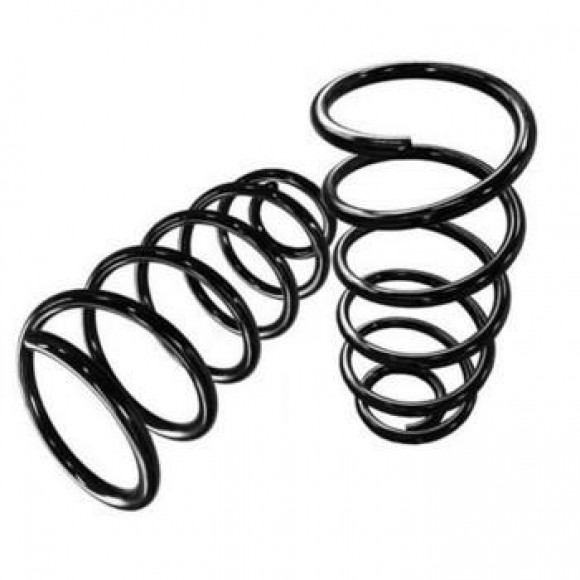
\includegraphics[width=0.5\textwidth]{molas_dianteiras_originais_150.jpg}
    \caption{Exemplo de um objeto elástico - uma mola}
    \label{fig:mola}
\end{figure}

O físico inglês Robert Hooke descobriu a relação da força que uma mola produz a partir da sua deformação:
\begin{equation}
    F_{el} = -kx
\end{equation}
\noindent em que $k$ é a \textbf{Constante de Deformação da mola} e $x$ é a deformação sofrida por uma mola, em que: $x=x_f - x_i$ ($x_f$ é o tamanho final da mola e $x_i$ é o tamanho natural da mola)

\textbf{O sinal negativo é porque a força tem direção oposta à deformação. Se a mola é comprimida $(x<0)$, a força será para expandir a mola $(F_{el} >0)$ e se ela for estendida $(x>0)$, a força será contrair a mola $(F_{el}<0)$}

A unidade de $k$ é: 
\begin{equation}
    [k] = \frac{N}{m} \quad ou \quad \frac{N}{cm}
\end{equation}

Pode ser que as informações sobre uma mola sejam dadas por um gráfico como a seguir:
\begin{figure}[h]
    \centering
    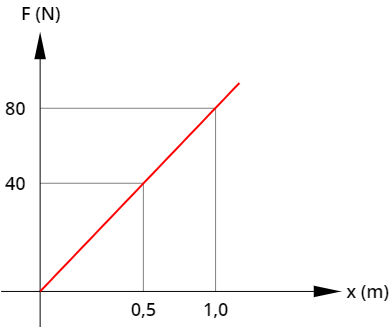
\includegraphics[width=0.3\textwidth]{grafico-hooke.jpg}
    \caption{Gráfico da força elástica de uma mola pela sua elongação}
    \label{fig:hooke}
\end{figure}

Com o gráfico, é possível achar a constante de deformação da mola por:
\begin{equation}
    k = \frac{y_2-y_1}{x_2-x_1}
\end{equation}
No exemplo do gráfico: $k= \frac{80-40}{1-0,5} = \frac{40}{0,5} = 80 N/m$

\textbf{Exemplo:} Uma mola de constante elástica igual a 200 N/m tem comprimento de 20 cm. Quando submetido a uma força externa, o comprimento dessa mola passa a ser de 15 cm. Determine o módulo da força elástica que é exercida pela mola, quando comprimida em 15 cm.
\textit{Solução:}
Como o comprimento natural da mola é de 20 cm e agora ela tem 15 cm, então a deformação é de:
\begin{align*}
    x = 15-20 = -5\,cm = -0,05\, m
\end{align*}

Então, a Lei de Hooke será:

\begin{align*}
    F_{el} = 200*(-0,05) = -10\,N
\end{align*}

\begin{itemize}
    \item \textbf{Associação de molas em série}
    Quando colocamos 2 molas, uma seguida da outra, como na figura a seguir:
    
    \begin{figure}[h]
        \centering
        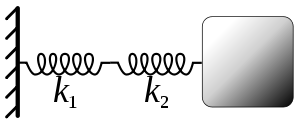
\includegraphics[width=0.5\textwidth]{300px-SpringsInSeries.svg.png}
        \caption{Esquema da associação de molas em série}
        \label{fig:serie}
    \end{figure}
    
        Podemos substituir o sistema por uma mola com uma constante de mola equivalente, que gere a mesma força. A constante de mola equivalente é dada por:
    \begin{equation}
        \frac{1}{k_{eq}} = \frac{1}{k_1} + \frac{1}{k_2}
    \end{equation}
    
    \item\textbf{Associação de molas em paralelo}
    Quando colocamos 2 molas, conectadas a um mesmo corpo como na figura a seguir:
    
    \begin{figure}[h]
        \centering
        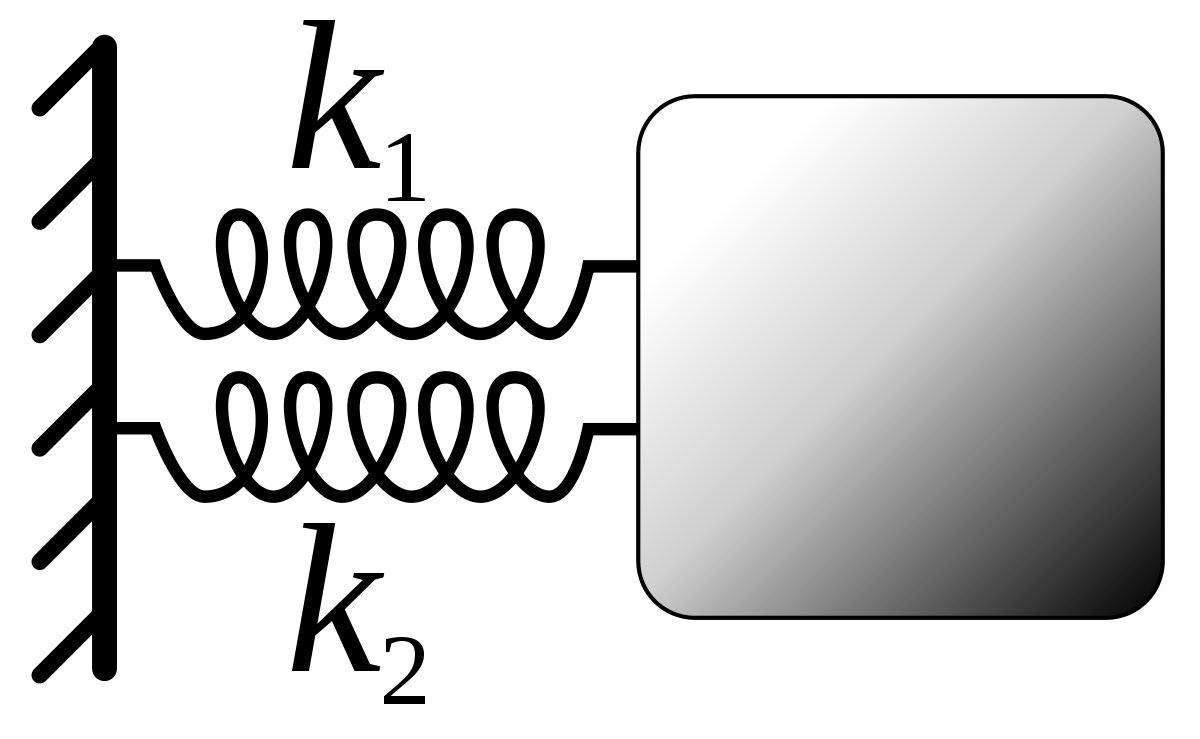
\includegraphics[width=0.5\textwidth]{1200px-SpringsInParallel.svg.png}
        \caption{Esquema da associação de molas em paralelo}
        \label{fig:serie}
    \end{figure}
    
    Podemos substituir o sistema por uma mola com uma constante de mola equivalente, que gere a mesma força. A constante de mola equivalente é dada por:
    \begin{equation}
        k_{eq} = k_1 + k_2
    \end{equation}
\end{itemize}

\subsection{Força de Tração no fio $\vec{T}$}

\textbf{É a força que um corpo sofre quando ele está pendurado por um fio.} Para um corpo que está parado e/ou não acelerando:
\begin{align}
    T = P = m*g
\end{align}
\noindent em que $m$ é a massa do objeto pendurado e $g$ é a aceleração da gravidade ($g = 10\,m/s^2$)

Um exemplo de tração é um fio sustentando uma bola de discoteca:

\begin{figure}[h]
    \centering
    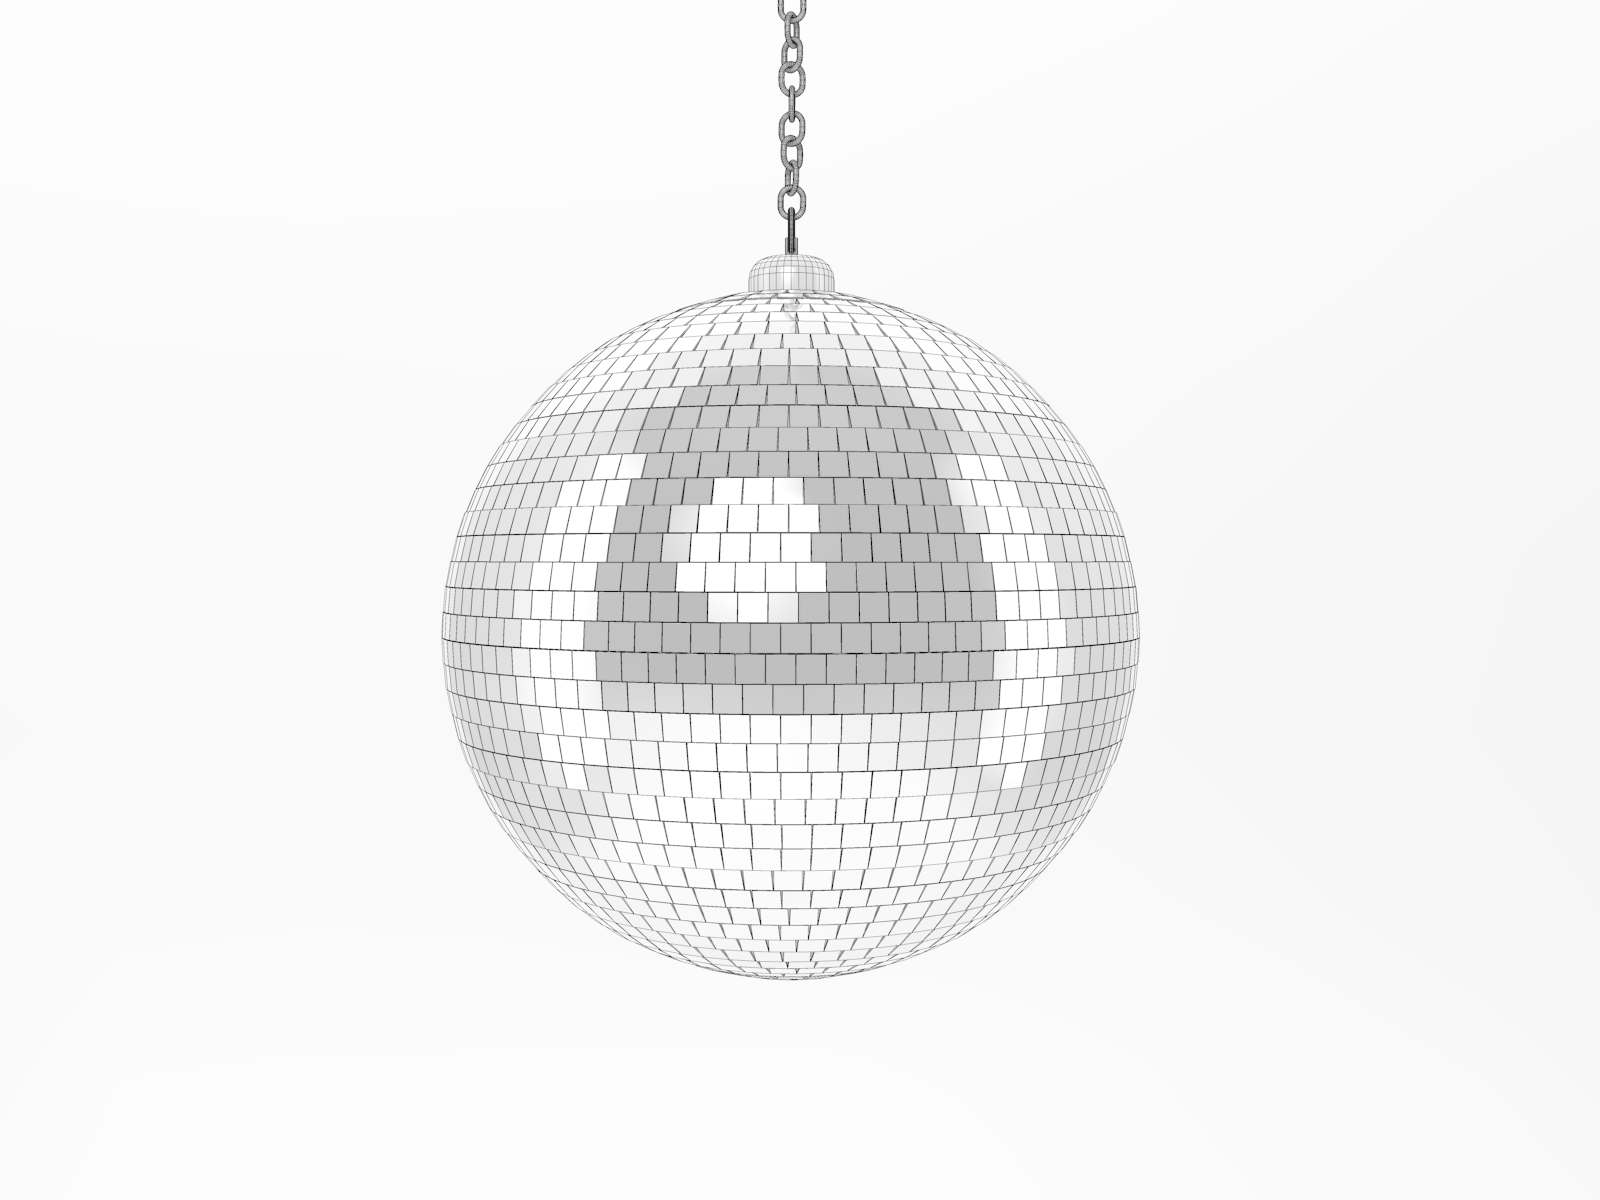
\includegraphics[width=0.5\textwidth]{discoball.png}
    \caption{Bola de discoteca. O fio que sustenta a bola aplica uma tração para cima, com a mesma intensidade da Força Peso, assim a bola fica parada.}
    \label{fig:my_label}
\end{figure}

Outro exemplo é a corda de um violão.
\begin{figure}[H]
    \centering
    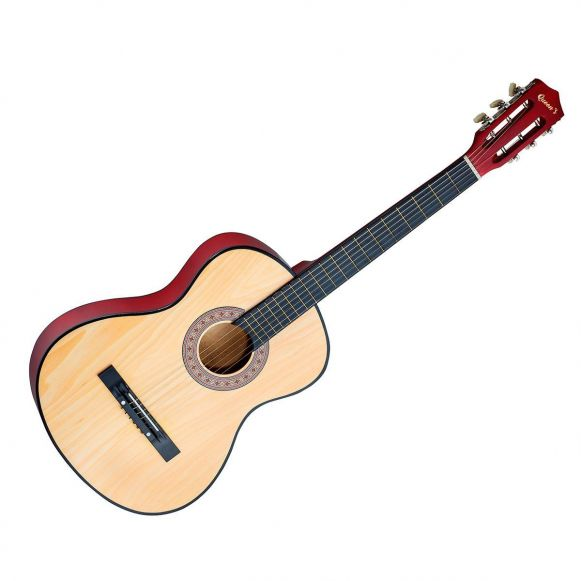
\includegraphics[width=0.5\textwidth]{violao-queens-com-cordas-de-aco-para-iniciante_261061_2.jpg}
    \caption{Imagem de um violão. As cordas dele sofrem uma tração igual nas duas pontas.}
    \label{fig:guitar}
\end{figure}

\textbf{Exemplo:} Suponha uma bola de massa de 500g pendurada por um fio preso no teto. Qual é a tração do fio, de forma que a bola não caia e fique pendurada?

\textit{Solução:} O esquema de forças da bola é dado por:
\begin{figure}[h]
    \centering
    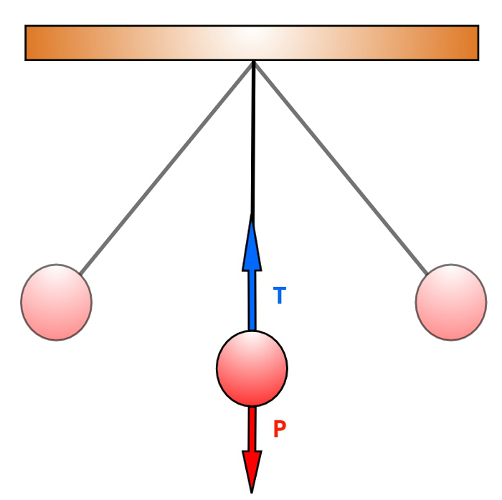
\includegraphics[width=0.4\textwidth]{tracao-no-pendulo.jpg}
    \label{fig:tracao}
\end{figure}

Para que a bola não cai, isso significa que a força resultante sobre a bola deva ser 0:
\begin{align*}
    F_{res} = P - T = 0\\
    m*g = T
\end{align*}
O sinal de '-' é porque convencionei que a direção positiva é para baixo. Colocando os dados:
\begin{align*}
    T = 0,5 *10 = 5N
\end{align*}

\subsection{Força Normal ($\vec{N}$)}

\textbf{É a força que uma superfície faz sobre um corpo quando este está em contato.} Essa força tem direção perpendicular à superfície. Caso a superfície seja horizontal, a força normal tem direção para cima:
\begin{figure}[h]
    \centering
    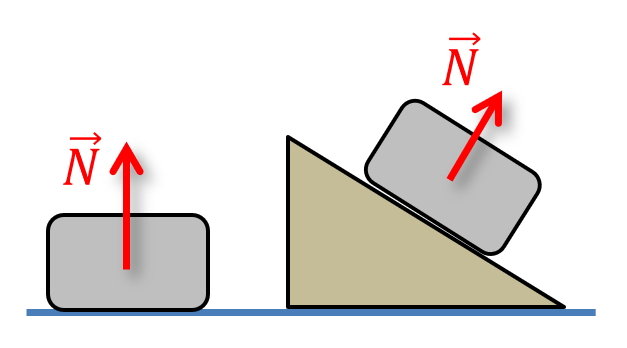
\includegraphics[width=0.5\textwidth]{word-image-1.png}
    \caption{Diagrama da força normal. Perceba que ela sempre é perpendicular à superfície. Nem sempre ela é para cima, ela pode ser para a diagonal. Isso será útil para futuras aulas!}
    \label{fig:normal}
\end{figure}

No exercício extra da aula de introdução à dinâmica, falei de um objeto de 70 kg que fica parado na superfície da Terra. Como o objeto está parado verticalmente, então a força resultante vertical no objeto é nula, logo tem que ter uma força que anula a força peso.

Como o objeto está sobre o chão, quem anula a força peso é a força normal. Podemos calculá-la como:
\begin{align*}
    F_{res} = P - N = 0\\
    70*10 - N =0 \implies N = 700 N
\end{align*}

A força que evita que a gente seja sugado para o centro da terra é a força normal e, \textbf{no caso de uma superfície horizontal, ela é dada como:}
\begin{equation}
    N = P = m*g
\end{equation}

\subsection{Força de atrito ($\vec{F}_{at}$)}

\textbf{Essa é a força quando um corpo tenta se movimentar/deslizar sobre uma superfície. A força tem direção oposta ao movimento e paralela a superfície. Ela faz o trabalho de freiar/segurar um objeto.}

Ela tem a seguinte forma:
\begin{equation}
    F_{at} = \mu *N
\end{equation}
\noindent em que $\mu$ (leia-se 'mi') é o \textbf{coeficiente de atrito.} Ele não tem unidade e varia de superfície para superfície. $N$ é a força normal, que acabamos de ver.

\textbf{Atenção:} nem sempre a força normal é vertical, então cuidado com o valor da força normal.

\begin{figure}[h]
    \centering
    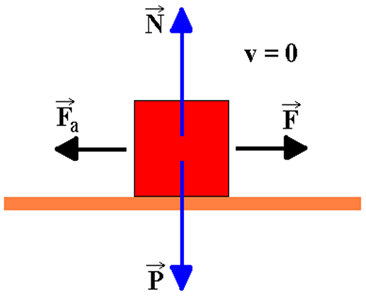
\includegraphics[width=0.5\textwidth]{bloco-parado.jpg}
    \caption{Diagrama de forças para um bloco sendo puxado sobre uma superfície. A força de atrito é oposta à direção que o bloco gostaria de se movimentar (na direção da força F)}
    \label{fig:my_label}
\end{figure}

\textbf{Exemplo}: Dado um corpo de 1 kg sobre uma superfície horizontal plana, com um diagrama igual à figura anterior. Supondo que a força F seja de 10 N e que o coeficiente de atrito seja 0,5. Qual é a força de atrito? Qual é a força e a aceleração resultante?

\textit{Solução:} Vamos separar o exercício em 2 partes: vertical e horizontal.

Na vertical, como o corpo não sobe nem desce: $F_r = 0$:
\begin{align*}
    &F_r^{vert} = P - N =0 \\
    &m*g = N \implies N = 1*10 = 10 N 
\end{align*}

Com a normal, podemos calcular a força de atrito:
\begin{align*}
    F_{at} = \mu*N = 0,5*10\implies \boxed{F_{at} = 5 N}
\end{align*}

Como verticalmente o corpo está parado, o corpo só pode se mover na horizontal. Tomando para a direita como a direção positiva, temos que:
\begin{align*}
    &F_r^{hor} = F - F_{at} = 10 - 5 \implies \boxed{F_r^{hor} = 5 N }\\
    &\boxed{F_r^{vert} = 0}
\end{align*}

Para achar a aceleração, vamos usar a Segunda Lei de Newton:
\begin{align*}
    F_r = m*a 
\end{align*}

Como só tem a força resultante diferente de 0 na horizontal:
\begin{align*}
    &F_r^{hor} = m*a \\
    &5=1*a \implies \boxed{a = 5\,m/s^2}
\end{align*}

\section{Equilíbrios}

Equilíbrio é quando um corpo está sob a ação de forças tal que o corpo não se movimente. Há 2 classificações de equílibrios:
\begin{enumerate}
    \item \textbf{Equílibrio estável} - é quando, mesmo que eu mude um pouco a posição do corpo, ele volta ao ponto inicial e fica parado lá. \textbf{Exemplo:} uma bola dentro de um buraco - mesmo que você mude um pouco a posição da bola no buraco, ela vai parar no fundo do buraco.
    
    \item \textbf{Equilíbrio instável} - é quando eu mudo um pouco a posição do corpo, ele não consegue voltar a posição de equilíbrio, ele vai para um outro lugar. \textbf{Exemplo:} uma bola sobre o topo do morro - qualquer toque na bola no topo de um morro, a bola começa a rolar e desce o morro.
\end{enumerate}
\begin{figure}[h]
    \centering
    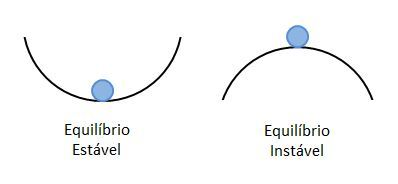
\includegraphics[width=0.5\textwidth]{equilibrios.jpg}
    \caption{Exemplos de equilíbrios estável e instável}
    \label{fig:equilibrium}
\end{figure}

\subsection{Equilíbrio Estático}
\textbf{É para os problemas em que os corpos estão parados, e mesmo sob ação de forças, eles permanecem parados.} A condição do equilíbrio estático é:
\begin{equation}
    \vec{F}_{res} =0
\end{equation}
\noindent $\vec{F}_{res}$ é a soma vetorial de todas as forças sobre um corpo. Podemos reescrever a equação acima em termos das forças horizontais e verticais:
\begin{equation}
    F_{res}^{vert} = 0 \quad \quad F_{res}^{hor} = 0
\end{equation}
\noindent em que $F_{res}^{vert},F_{res}^{hor}$ é a força resultante na parte vertical e na parte horizontal, respectivamente.

Isso é muito importante para prédios na engenharia civil, por exemplo, em que se constrói prédios de forma que eles não se movimentem, então a soma de todas as forças que um prédio sofre tem que ser zero.

\subsection{Equilíbrio Dinâmico}
\textbf{É para os problemas em que os corpos estão em movimento e mesmo sob ação de forças, eles permanecem fazendo o movimento inicial.}A condição do equilíbrio dinâmico é:
\begin{equation}
    \vec{F}_{res} =0
\end{equation}
\noindent $\vec{F}_{res}$ é a soma vetorial de todas as forças sobre um corpo. Podemos reescrever a equação acima em termos das forças horizontais e verticais:
\begin{equation}
    F_{res}^{vert} = 0 \quad \quad F_{res}^{hor} = 0
\end{equation}
\noindent em que $F_{res}^{vert},F_{res}^{hor}$ é a força resultante na parte vertical e na parte horizontal, respectivamente.

Pessoal da Engenharia aeroespacial estuda bastante sobre o equilíbrio dinâmico para o design de asas dos aviões de forma que o avião não caia e continua a plainar.

\end{document}
